On a ajouté au modèle SimplePDL la gestion des ressources.
Pour celà, on a introduit :
\begin{itemize}
\item Ressource : une ressource ayant un nom et étant présente en une certaine quantité
\item Need : un besoin représentant un nombre de ressources d'un certain type
\item NeedSet : un ensemble de besoins nécessaires à la réalisation d'une WD
\end{itemize}

\vspace{1em}
Voilà un diagramme représentant le métamodèle SimplePDL que j'ai utilisé :
\begin{center}
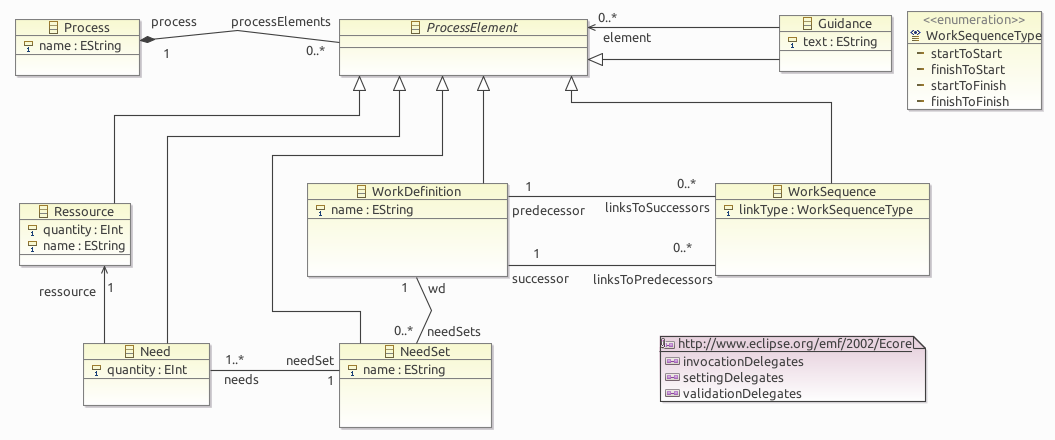
\includegraphics[width=\textwidth]{../Images/meta_pdl.png}
\end{center}

\newpage
Ce modèle n'est pas suffisant pour décrire entièrement l'ensemble des contraintes. Pour celà on a donc ajouté des contraintes OCL avec OCLinEcore.\\

On a ajouté les règles suivantes :
\begin{itemize}
\item class Process
\begin{itemize}
\item sameWDName : les WD doivent avoir des noms différents
\item sameRessourcesName : les ressources doivent avoir des noms différents
\item nameForbidden : un processus ne peut pas s'appeler : "Process"
\item sameNeedSetsName :
\end{itemize}

\item class WorkDefinition
\begin{itemize}
\item voidName : nom vide interdit
\end{itemize}

\item class WorkSequence
\begin{itemize}
\item previousWDinSameProcess : la WD précédente doit être dans le même processus
\item reflexivity : le prédécesseur et le successeur oivent être différents
\item nextWDinSameProcess : la WD suivante doit être dans le même processus
\end{itemize}

\item class Ressource
\begin{itemize}
\item voidName : nom vide interdit
\item positiveQuantity : la quantité de ressources doit être >= 0
\end{itemize}

\item class Need
\begin{itemize}
\item positiveQuantity : la quantité de ressources d'un besoin doit être > 0
\end{itemize}

\item class NeedSet
\begin{itemize}
\item voidName : nom vide interdit
\end{itemize}
\end{itemize}
